% ============================================================================
%  REPORTE FINAL — Almacenes y Minería de Datos (UNAM)
%  Proyecto: Triage de reportes de incidentes viales del C5 (CDMX 2022-2024)
%
%  Compilar:  cd reports && pdflatex reporte.tex   (córrelo 2 veces para el índice)
%  Las cifras provienen de los tres notebooks ejecutados (01_eda, 
%  02_clasificacion y 03_clustering).
% ============================================================================
\documentclass[11pt,letterpaper]{article}

\usepackage[utf8]{inputenc}
\usepackage[T1]{fontenc}
\usepackage[spanish,es-nodecimaldot]{babel}
\usepackage{lmodern}
\usepackage[margin=2.5cm]{geometry}
\usepackage{graphicx}
\usepackage{booktabs}
\usepackage{array}
\usepackage{longtable}
\usepackage{xcolor}
\usepackage{enumitem}
\usepackage{caption}
\usepackage{amsmath}
\usepackage{float}
\usepackage{tikz}
\usetikzlibrary{arrows.meta, positioning, shapes.geometric, calc}
\usepackage[hidelinks]{hyperref}

\graphicspath{{../figures/}}

% Marca para lo que falta completar (se ve en rojo en el PDF)
\newcommand{\TODO}[1]{\textcolor{red}{\textbf{[POR COMPLETAR: #1]}}}

\captionsetup{font=small,labelfont=bf}

\begin{document}

% ============================================================================
% 1. PORTADA
% ============================================================================
\begin{titlepage}
\centering
\vspace*{1.5cm}
{\scshape\large Universidad Nacional Autónoma de México\par}
{\scshape Facultad de Ciencias\par}
\vspace{0.5cm}
{\scshape Almacenes y Minería de Datos\par}
\vspace{2.5cm}

\rule{\linewidth}{0.4pt}\\[0.4cm]
{\huge\bfseries Triage de reportes de incidentes viales del C5\par}
\vspace{0.3cm}
{\Large ¿Es real o falso un reporte vial? Predicción de veracidad y\\
descubrimiento de corredores de incidentes en la Ciudad de México\par}
\rule{\linewidth}{0.4pt}\\[1.5cm]

{\large\bfseries Proyecto Final\par}
\vspace{2cm}

{\large
\begin{tabular}{ll}
\textbf{Integrante:} & José Rubén Alfaro González\\
                     & No.\ de cuenta: 320516436\\
\end{tabular}\par}

\vspace{1.5cm}
{\large Profesora: Jessica Santizo Galicia\par}
{\normalsize Ayudante de Teoría: Diego Antonio Villalba González\par}
{\normalsize Ayudante de Laboratorio: Ares Gael Castro Romero\par}

\vfill
{\large Ciudad de México, junio de 2026\par}
\end{titlepage}

\tableofcontents
\newpage

% ============================================================================
% 2. INTRODUCCIÓN
% ============================================================================
\section{Introducción}

\textbf{Problema.} El Centro de Comando, Control, Cómputo, Comunicaciones y
Contacto Ciudadano (C5) de la Ciudad de México recibe cientos de miles de
reportes de incidentes viales al año a través de distintos canales (llamadas al
911, botones de auxilio, cámaras, radio). Una fracción importante de esos
reportes no corresponde a un incidente confirmado: son falsos o meramente
informativos. Despachar unidades de emergencia a reportes que no lo ameritan
desperdicia recursos escasos y retrasa la atención de incidentes reales.

\textbf{Objetivo.} Construir un modelo que, con la información disponible
\emph{al momento de recibir un reporte} (canal de entrada, tipo de incidente,
hora, alcaldía y ubicación), estime la probabilidad de que sea un incidente
real (confirmado, ``afirmativo'') frente a falso/informativo, para apoyar la
priorización del despacho; y, de forma complementaria, identificar mediante
agrupamiento espacial las \emph{vialidades} donde se concentran los incidentes
y de qué tipo, como insumo para la planeación operativa.

\textbf{Justificación y valor.} En nuestro conjunto de datos, el 36.5\,\% de
los reportes viales no duplicados que recibe el C5 termina cerrándose como
falso o informativo: más de uno de cada tres despachos potenciales no
corresponde a un incidente verificable. En una ciudad donde las unidades de
emergencia son un recurso finito, cada despacho innecesario tiene un costo de
oportunidad directo sobre los incidentes verdaderos, cuya atención oportuna
puede ser cuestión de vida o muerte (la literatura documenta el papel central
de las llamadas de emergencia relacionadas con tránsito en la CDMX
\cite{melgoza}). Un modelo de triage que ordene los reportes entrantes por su
probabilidad de ser reales permite priorizar el despacho con evidencia,
concentrar la verificación humana en los casos ambiguos y dimensionar el
problema de las falsas alarmas. El análisis es, además, completamente
reproducible sobre datos públicos oficiales.

% ============================================================================
% 3. DESCRIPCIÓN DEL DATASET
% ============================================================================
\section{Descripción del dataset}

\textbf{Fuente.} Conjunto de datos abiertos ``Incidentes viales reportados por
el C5'' del Portal de Datos Abiertos de la Ciudad de México
(\url{https://datos.cdmx.gob.mx}), publicado por el propio C5 bajo licencia
CC-BY-4.0. Corte 2022--2024, descargado en junio de 2026. La fuente es de uso
académico reconocido: estudios recientes sobre siniestralidad vial en la CDMX
la emplean explícitamente como una de sus fuentes primarias
\cite{herreraortiz}.

\textbf{Tamaño.} El archivo crudo contiene 504\,261 reportes; tras la
preparación (Sección~\ref{sec:limpieza}) el conjunto de trabajo queda en
\textbf{289\,885 reportes y 18 variables}, con mezcla de variables numéricas y
categóricas.

\textbf{Variables.} El diccionario completo (significado, tipo, valores
posibles y rol de cada variable) está en \texttt{reports/diccionario\_datos.md}
y en el notebook \texttt{01\_eda.ipynb}. La Tabla~\ref{tab:dic} resume las
principales.

\begin{table}[H]
\centering
\caption{Variables principales (diccionario resumido).}
\label{tab:dic}
\small
\begin{tabular}{@{}lll@{}}
\toprule
\textbf{Variable} & \textbf{Tipo} & \textbf{Descripción / valores} \\
\midrule
\texttt{codigo\_cierre} & cat. & A=Afirmativo, D=Duplicado, F=Falso, I=Informativo (base del target)\\
\texttt{REAL} & 0/1 & \textbf{Target}: 1 si afirmativo, 0 si falso/informativo\\
\texttt{tipo\_entrada} & cat. (9) & Canal: llamada del 911, botón de auxilio, cámara, radio, \dots\\
\texttt{incidente\_c4} & cat. (16) & Choque s/lesionados, choque c/lesionados, atropellado, \dots\\
\texttt{tipo\_incidente\_c4} & cat. (7) & Accidente, lesionado, cadáver, \dots\\
\texttt{alcaldia\_catalogo} & cat. (16) & Las 16 alcaldías de la CDMX\\
\texttt{HORA, FRANJA, dia\_semana, MES, ANIO} & num./cat. & Variables temporales del reporte\\
\texttt{latitud, longitud} & num. & Ubicación del incidente\\
\texttt{TIEMPO\_CIERRE\_MIN} & num. & Minutos hasta el cierre (\emph{fuga}: excluida del modelo)\\
\texttt{clas\_con\_f\_alarma} & cat. & Clasificación posterior al cierre (\emph{fuga}: excluida del modelo)\\
\bottomrule
\end{tabular}
\end{table}

\textbf{Limitaciones conocidas.} (i) El etiquetado de veracidad es
\emph{institucional}: refleja los criterios de cierre del C5, no una
verificación independiente; cualquier sesgo de ese proceso lo hereda el
modelo. (ii) La llamada del 911 concentra el 87.6\,\% del volumen, de modo que
el desempeño global está dominado por el canal más ambiguo. (iii) La
geocodificación es incompleta en una fracción mínima (366 reportes sin
alcaldía, 0.13\,\%). (iv) La ventana temporal es 2022--febrero de 2024, por lo
que los patrones podrían no extrapolar a periodos con dinámicas distintas.
(v) No se dispone de variables de contexto (clima, tráfico, contenido de la
llamada) que probablemente elevarían el techo de predicción.

% ============================================================================
% 4. LIMPIEZA Y PREPARACIÓN DE DATOS
% ============================================================================
\section{Limpieza y preparación de datos}
\label{sec:limpieza}

La preparación se implementó con el \textbf{patrón de diseño Pipeline}: una
secuencia de pasos atómicos (cada uno una función
\texttt{df}$\rightarrow$\texttt{df}) encadenados por una clase
\texttt{PipelinePreparacion} que registra una bitácora auditable de filas
antes/después de cada paso (notebook \texttt{01\_eda.ipynb}, sección 2).

\begin{table}[H]
\centering
\caption{Bitácora del pipeline de preparación.}
\label{tab:pipe}
\small
\begin{tabular}{@{}lrr@{}}
\toprule
\textbf{Paso} & \textbf{Filas antes} & \textbf{Filas después}\\
\midrule
\texttt{quitar\_duplicados} & 504\,261 & 289\,935\\
\texttt{quitar\_anio\_ruido} & 289\,935 & 289\,885\\
\texttt{construir\_target} & 289\,885 & 289\,885\\
\bottomrule
\end{tabular}
\end{table}

\textbf{Decisión clave — eliminación de duplicados.} La distribución del
cierre en el crudo es: D (duplicado) 42.5\,\%, A (afirmativo) 36.5\,\%, F
(falso) 20.3\,\%, I (informativo) 0.7\,\%. Un reporte con cierre \texttt{D}
corresponde a un \emph{evento real} que ya fue reportado antes. Como el
objetivo del modelo es distinguir reportes reales de falsos, y la
deduplicación (verificar si ya hay una unidad en el sitio) es responsabilidad
del \emph{sistema de despacho} y no del modelo de veracidad, los duplicados se
eliminan. El target se define sobre los reportes no duplicados:
\texttt{REAL}=1 si el cierre es afirmativo (\texttt{A}), 0 si es falso
(\texttt{F}) o informativo (\texttt{I}). Se descartó la alternativa de contar
los duplicados como reales porque produce un balance mucho peor
($\sim$79/21) y un target conceptualmente borroso (mezcla ``confirmado'' con
``ya reportado'').

\textbf{Otras decisiones.} (i) El segundo paso elimina 50 reportes de
diciembre de 2021 que se colaron en el corte (ruido de frontera). (ii)
\emph{Faltantes}: solo tres columnas tienen nulos y todos son marginales
—\texttt{alcaldia\_catalogo} 366 (0.13\,\%), \texttt{tipo\_entrada} 3,
\texttt{TIEMPO\_CIERRE\_MIN} 2—; no se eliminan filas: el
\texttt{ColumnTransformer} del modelo los imputa con la categoría más
frecuente. (iii) \emph{Duplicados exactos}: tras retirar los cierres
\texttt{D} no queda ningún folio repetido ni fila idéntica. (iv)
\emph{Outliers}: la regla IQR sobre \texttt{TIEMPO\_CIERRE\_MIN} marca 49\,211
reportes (17.0\,\%) por encima del límite superior (287.5 min); no se eliminan
porque son tiempos de servicio \emph{reales} (casos complejos que tardan en
cerrarse), no errores de captura, y porque esa columna no es variable del
modelo. (v) \emph{Anti-fuga}: \texttt{TIEMPO\_CIERRE\_MIN} y
\texttt{clas\_con\_f\_alarma} se conservan en el dataset solo para análisis;
quedan excluidas del modelo (Sección~\ref{sec:modelo}).

% ============================================================================
% 5. ANÁLISIS EXPLORATORIO
% ============================================================================
\section{Análisis Exploratorio de Datos (EDA)}

\subsection{Balance del target}

Tras la preparación, el 63.5\,\% de los reportes son reales (cierre
afirmativo) y el 36.5\,\% falsos/informativos: un desbalance moderado de
1.74:1 (Figura~\ref{fig:balance}). De aquí se derivan dos decisiones de
modelado: la métrica rectora es el \textbf{F1 macro} —la \emph{accuracy} la
alcanzaría casi un clasificador trivial que diga ``real'' a todo— y el bosque
usa \texttt{class\_weight='balanced'} para no sacrificar el recall de la clase
minoritaria, pues detectar reportes falsos es justamente el valor de negocio.

\begin{figure}[H]\centering
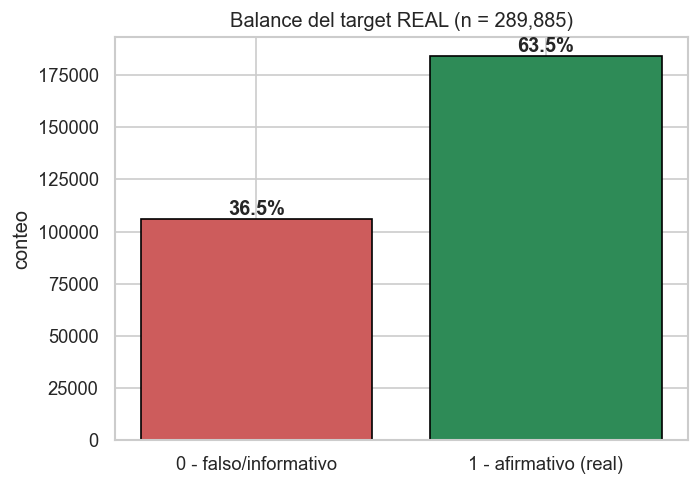
\includegraphics[width=0.55\linewidth]{01_balance_target.png}
\caption{Balance del target \texttt{REAL} en el conjunto depurado (289\,885 reportes).}
\label{fig:balance}
\end{figure}

\subsection{Estadística descriptiva y valores atípicos}

Para las dos numéricas más informativas se reportó media, mediana, desviación,
cuartiles, rango y forma. \texttt{HORA} es casi simétrica (asimetría $-0.52$,
curtosis $-0.58$; mediana 15\,h): los reportes se reparten a lo largo del día
con concentración vespertina. En cambio \texttt{TIEMPO\_CIERRE\_MIN} está
fuertemente sesgada a la derecha (asimetría 3.7, curtosis 15.5): mediana de
$\sim$189 minutos con una cola que llega a 4\,657. La regla IQR marca 17.0\,\%
de atípicos en esa cola (límite superior 287.5 min); se conservan por ser
tiempos de servicio reales —casos complejos que tardan en cerrarse— y porque
la variable queda fuera del modelo por fuga. Esta forma extrema, típica de
tiempos de servicio, ilustra por qué los atípicos deben evaluarse en su
contexto y no eliminarse mecánicamente.

\subsection{Distribuciones temporales}

La Figura~\ref{fig:dist} muestra los ritmos de la ciudad: pocos reportes de
madrugada (3--6\,h), ascenso matutino y el grueso entre la tarde y la noche;
por día de la semana destacan viernes y sábado (mayor movilidad y vida
nocturna) y el lunes es el día más tranquilo. Son patrones plausibles que
aportan señal temporal moderada al modelo.

\begin{figure}[H]\centering
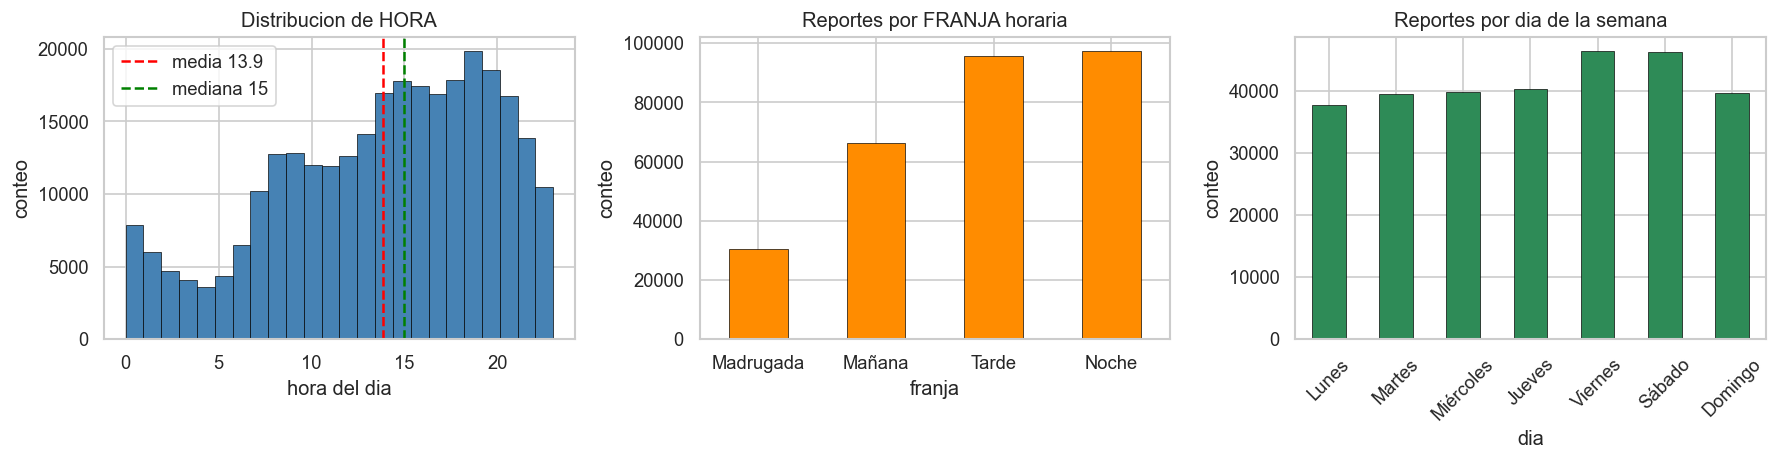
\includegraphics[width=\linewidth]{01_distribuciones.png}
\caption{Distribución de reportes por hora del día, franja horaria y día de la semana.}
\label{fig:dist}
\end{figure}

\subsection{Geografía del reporte: ¿quién reporta y qué tan confiable es?}

\textbf{Por canal de entrada.} Es el hallazgo central del EDA
(Figura~\ref{fig:canal}). Los canales \emph{institucionales} operados por
personal del C5 confirman casi siempre: radio 93.3\,\%, cámara 92.9\,\% y
botón de auxilio 88.4\,\%. La llamada del 911 —que concentra el 87.6\,\% del
volumen— confirma solo 59.8\,\%, y los aplicativos ciudadanos apenas
28.4\,\%. La implicación operativa es directa: lo que entra por canales
institucionales puede despacharse casi automáticamente con alta prioridad,
mientras que el escrutinio debe concentrarse en la avalancha de llamadas
ciudadanas, donde vive la ambigüedad.

\begin{figure}[H]\centering
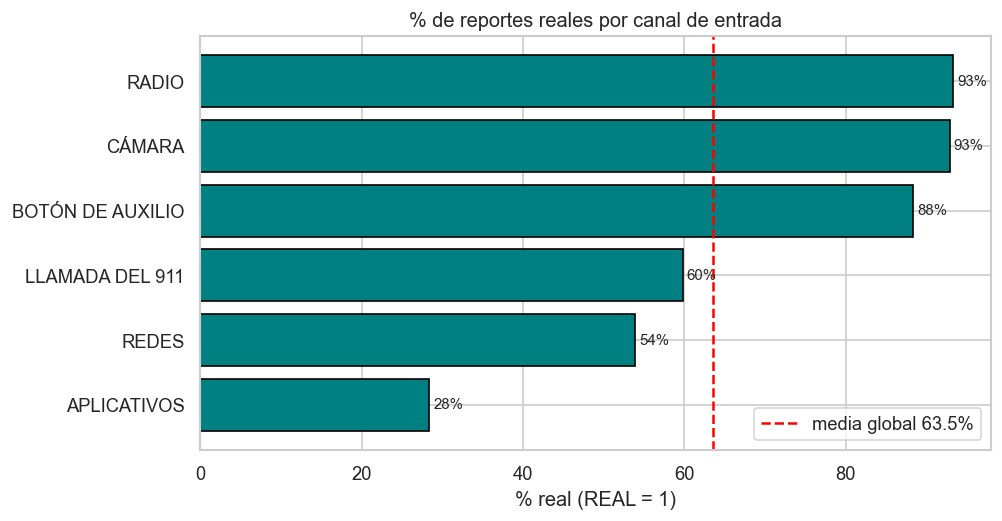
\includegraphics[width=0.78\linewidth]{01_fuente_confirmacion.png}
\caption{Tasa de confirmación (\% de reportes reales) por canal de entrada.}
\label{fig:canal}
\end{figure}

\textbf{Por alcaldía.} El ranking va de Cuauhtémoc (75.3\,\%) y Azcapotzalco
(72.4\,\%) hasta Xochimilco (51.8\,\%) y Cuajimalpa (50.7\,\%): un rango de
$\sim$25 puntos (Figura~\ref{fig:alcaldia}). Las alcaldías centrales —con más
cámaras, operadores y tráfico verificable— tienden a mayor confirmación que la
periferia. La brecha es real pero menor que la del canal ($\sim$33 puntos): la
geografía aporta señal complementaria.

\begin{figure}[H]\centering
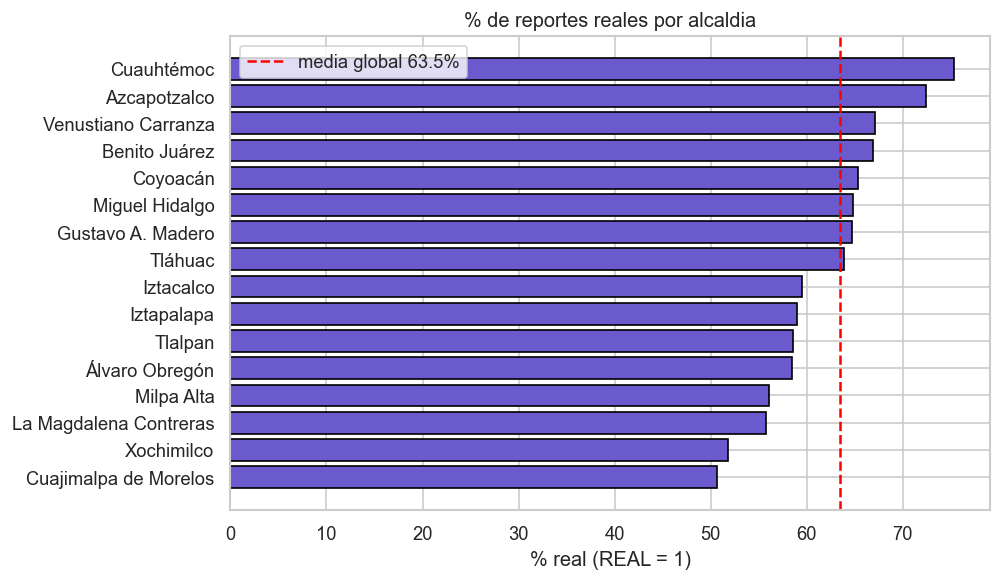
\includegraphics[width=0.78\linewidth]{01_alcaldia_confirmacion.png}
\caption{Tasa de confirmación por alcaldía.}
\label{fig:alcaldia}
\end{figure}

\textbf{Mezcla canal $\times$ alcaldía.} La prueba $\chi^2$ rechaza la
independencia ($\chi^2 = 3\,719.8$, gl $= 120$, $p \approx 0$), pero con
$n \approx 290$\,k casi cualquier asociación resulta ``significativa'': lo
informativo es el tamaño de efecto, y la V de Cramér $= 0.040$ es muy pequeña.
La cámara pesa más en alcaldías centrales y el botón de auxilio en la
periferia, pero el dominio de la llamada del 911 (entre el 80\,\% y el 95\,\% del
volumen según la alcaldía) homogeneiza la mezcla. Es un buen ejemplo de que
\emph{estadísticamente significativo} $\neq$ \emph{efecto grande}.

\textbf{Por franja horaria.} La confiabilidad decae a lo largo del día
(Figura~\ref{fig:franja}): madrugada 70.1\,\% y mañana 68.3\,\% superan la
media global (63.5\,\%), mientras tarde (61.5\,\%) y noche (60.1\,\%) quedan
por debajo —una brecha de 10 puntos. El detalle operativo es que tarde y noche
concentran además el mayor volumen (33.1\,\% y 33.6\,\%): las horas con más
reportes son justamente las de menor proporción de incidentes reales. El
patrón es coherente con el perfil horario de los canales: en horas valle la
vigilancia institucional (que confirma $\sim$90\,\%) sostiene una proporción
mayor del reporte, y la madrugada hereda parte de esa confiabilidad.

\begin{figure}[H]\centering
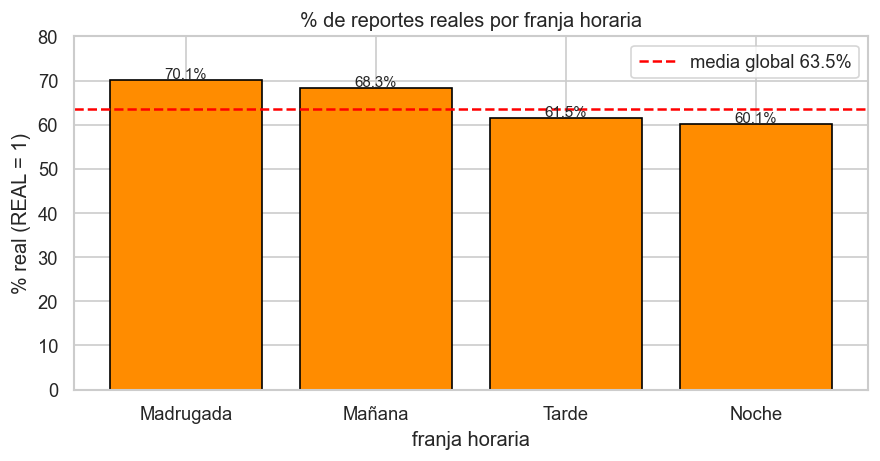
\includegraphics[width=0.62\linewidth]{01_franja_confirmacion.png}
\caption{Tasa de confirmación por franja horaria.}
\label{fig:franja}
\end{figure}

\subsection{Síntesis del EDA}

\begin{itemize}[nosep]
  \item Target con desbalance moderado (63.5/36.5) $\Rightarrow$ F1 macro como
        métrica rectora y pesos de clase balanceados.
  \item El \textbf{canal de entrada} separa fuertemente la veracidad
        (institucionales $\sim$90\,\% vs.\ 911 $\sim$60\,\%); se anticipa como
        variable clave del modelo.
  \item La \textbf{alcaldía} (rango 25 pts) y la \textbf{franja horaria}
        (rango 10 pts) aportan señal complementaria.
  \item Calidad de datos alta: faltantes marginales ($\leq$ 0.13\,\%), sin
        duplicados tras la preparación; atípicos de tiempos de cierre
        documentados y justificados (no eliminados).
  \item Frontera anti-fuga explícita: lo que se conoce \emph{al cerrar} el
        reporte no entra al modelo.
\end{itemize}

% ============================================================================
% 6. MODELO SUPERVISADO
% ============================================================================
\section{Modelo supervisado}
\label{sec:modelo}

\subsection{Variable objetivo y variables de entrada}

Se predice \texttt{REAL} (afirmativo vs.\ falso/informativo) usando
\emph{únicamente información disponible al recibir el reporte}: numéricas
(\texttt{HORA}, \texttt{MES}, \texttt{ANIO}, \texttt{latitud},
\texttt{longitud}) y categóricas (\texttt{tipo\_incidente\_c4},
\texttt{incidente\_c4}, \texttt{tipo\_entrada}, \texttt{alcaldia\_catalogo},
\texttt{dia\_semana}, \texttt{FRANJA}). Se excluyen por fuga de información
las columnas que solo se conocen tras el cierre (\texttt{TIEMPO\_CIERRE\_MIN}
y \texttt{clas\_con\_f\_alarma}, cuya categoría ``FALSA ALARMA'' es
prácticamente el target) y los identificadores (\texttt{folio},
\texttt{codigo\_cierre}, \texttt{CIERRE\_DESC}, \texttt{FECHA\_CREACION}). El
efecto de la fuga se cuantifica en la Sección~\ref{sec:fuga}.

\subsection{Proceso}

\textbf{Patrón Pipeline a nivel de modelo.} El clasificador se arma como un
\texttt{Pipeline} de \texttt{scikit-learn} \cite{sklearn} que encadena el
preprocesamiento y el estimador en un solo objeto:
\texttt{ColumnTransformer} con imputación por moda + \emph{one-hot}
(\texttt{handle\_unknown='ignore'}) para las categóricas y paso directo para
las numéricas (un bosque corta por umbrales: no necesita escalado), seguido de
un \texttt{RandomForestClassifier} \cite{rf} con 300 árboles,
\texttt{class\_weight='balanced'} y semilla 42. Esto garantiza que el mismo
preprocesamiento se aplique de forma idéntica en entrenamiento, validación y
predicción.

\textbf{Partición.} 80/20 estratificada por el target con semilla fija:
231\,908 reportes de entrenamiento y 57\,977 de prueba (balance 63.5/36.5 en
ambos lados).

\textbf{Ajuste de hiperparámetros.} \texttt{GridSearchCV} (validación cruzada
estratificada de 3 pliegues, métrica F1 macro) sobre una submuestra
estratificada de 80\,000 reportes del entrenamiento, explorando profundidad y
tamaño mínimo de hoja (Tabla~\ref{tab:tuning}). La mejor configuración
(\texttt{max\_depth}$=20$, \texttt{min\_samples\_leaf}$=1$) se reentrenó sobre
el entrenamiento completo antes de la evaluación final.

\begin{table}[H]
\centering
\caption{Búsqueda de hiperparámetros (F1 macro, validación cruzada sobre submuestra de 80k).}
\label{tab:tuning}
\small
\begin{tabular}{@{}ccc@{}}
\toprule
\texttt{max\_depth} & \texttt{min\_samples\_leaf} & \textbf{F1 macro (CV)}\\
\midrule
20   & 1  & \textbf{0.6566}\\
20   & 20 & 0.6548\\
None & 20 & 0.6546\\
None & 1  & 0.6207\\
\bottomrule
\end{tabular}
\end{table}

\subsection{Resultados}

La Tabla~\ref{tab:modelos} compara el modelo contra la línea base obligatoria
(clasificador de clase mayoritaria) y contra una red neuronal entrenada como
comparación (Sección~\ref{sec:mlp}).

\begin{table}[H]
\centering
\caption{Comparación de modelos en el conjunto de prueba (57\,977 reportes).}
\label{tab:modelos}
\small
\begin{tabular}{@{}lcccc@{}}
\toprule
\textbf{Modelo} & \textbf{Accuracy} & \textbf{F1 macro} & \textbf{F1 pond.} & \textbf{AUC}\\
\midrule
Línea base (mayoritario) & 0.635 & 0.388 & 0.493 & 0.500\\
\textbf{Random Forest (final)} & 0.670 & \textbf{0.658} & 0.675 & \textbf{0.729}\\
Red neuronal (MLP) & 0.686 & 0.638 & 0.674 & 0.726\\
\bottomrule
\end{tabular}
\end{table}

\textbf{Comparación con la línea base (obligatoria).} La línea base predice
``real'' para todo: alcanza 63.5\,\% de \emph{accuracy} pero un F1 macro de
0.388 y no detecta \emph{ningún} reporte falso, lo que la vuelve inservible
para filtrar el ruido operativo. El Random Forest sube el F1 macro a 0.658
($+0.27$) deteniendo una fracción sustancial de los falsos: el modelo aprende
señal genuina y supera con holgura el piso trivial.

\textbf{Métricas completas del Random Forest.} Accuracy 0.6700; precisión /
recall / F1 \emph{macro}: 0.6578 / 0.6684 / 0.6581; \emph{ponderadas}:
0.6898 / 0.6700 / 0.6753; AUC 0.7289. El desglose por clase
(Tabla~\ref{tab:clases}) muestra el equilibrio logrado con
\texttt{class\_weight='balanced'}: el recall de la clase minoritaria (falsos)
llega a 0.66 sin colapsar el de los reales (0.67).

\begin{table}[H]
\centering
\caption{Desglose por clase del Random Forest (conjunto de prueba).}
\label{tab:clases}
\small
\begin{tabular}{@{}lcccc@{}}
\toprule
\textbf{Clase} & \textbf{Precisión} & \textbf{Recall} & \textbf{F1} & \textbf{Soporte}\\
\midrule
Falso/Informativo (0) & 0.539 & 0.663 & 0.594 & 21\,164\\
Real/Afirmativo (1)   & 0.777 & 0.674 & 0.722 & 36\,813\\
\bottomrule
\end{tabular}
\end{table}

\begin{figure}[H]\centering
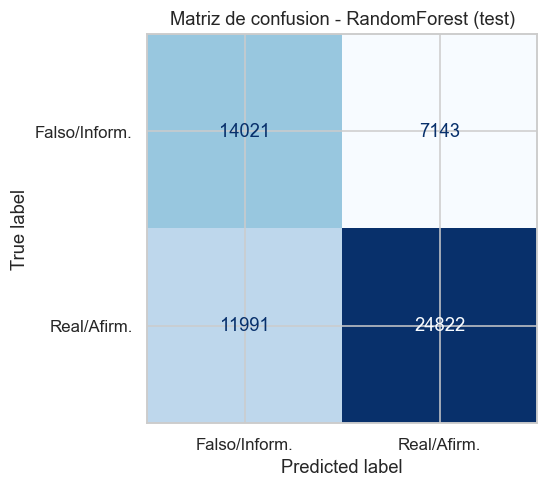
\includegraphics[width=0.46\linewidth]{02_matriz_confusion.png}\hfill
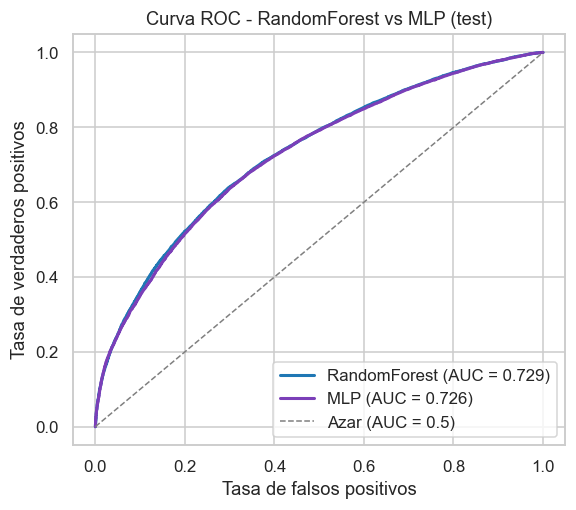
\includegraphics[width=0.50\linewidth]{02_curva_roc_mlp.png}
\caption{Izquierda: matriz de confusión del Random Forest. Derecha: curvas ROC
del Random Forest (AUC $=0.729$) y de la MLP (AUC $=0.726$).}
\label{fig:cmroc}
\end{figure}

\textbf{Interpretación.} En la matriz de confusión la diagonal concentra la
mayoría de los casos; los \emph{falsos negativos} (reportes reales
clasificados como falsos) son el error operativamente más costoso y se
analizan más abajo. Ambas curvas ROC se despegan claramente del azar; el AUC
moderado ($\sim$0.73) refleja el techo de separabilidad que impone la
información disponible al momento del reporte: hay señal real y aprovechable,
pero el problema no es trivialmente separable.

\subsection{Importancia de variables}

La importancia por permutación (muestra de 20\,000 reportes de prueba, 5
repeticiones, métrica F1 macro; Figura~\ref{fig:imp}) la dominan
\texttt{incidente\_c4} (0.102) y \texttt{tipo\_entrada} (0.031), muy por
encima del resto ($\leq 0.006$). Es decir: \emph{qué} se reporta y \emph{por
qué canal} predice la veracidad mejor que \emph{cuándo} o \emph{dónde}. El
resultado es coherente con el EDA: una cámara o un botón de auxilio suelen ir
asociados a eventos confirmados, mientras que la llamada del 911 es mucho más
heterogénea.

\begin{figure}[H]\centering
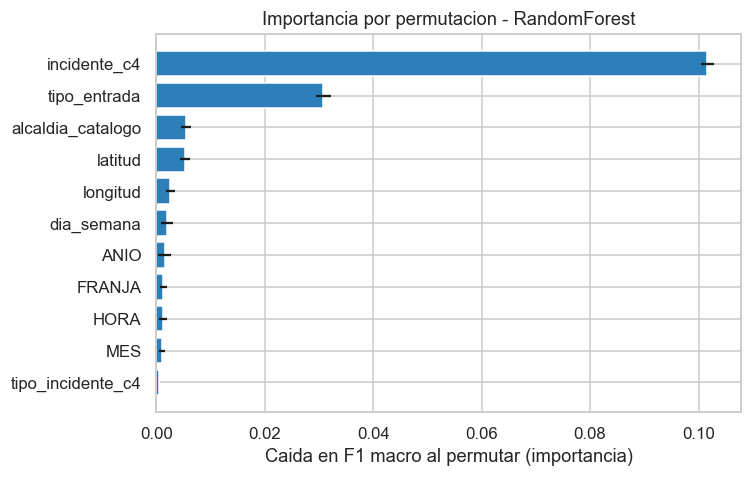
\includegraphics[width=0.72\linewidth]{02_importancia_permutacion.png}
\caption{Importancia por permutación del Random Forest (caída del F1 macro al
permutar cada variable original).}
\label{fig:imp}
\end{figure}

\subsection{Análisis de errores}

La tasa de error por canal (Tabla~\ref{tab:errores}) confirma dónde vive la
incertidumbre: la llamada del 911 se equivoca en el 36.3\,\% de los casos,
mientras los canales verificados son mucho más predecibles (cámara 8.7\,\%,
radio 7.1\,\%). De los 11\,991 falsos negativos —reportes reales clasificados
como falsos, el error operativamente más grave— la inmensa mayoría proviene
del 911, que es a la vez el canal más voluminoso y el menos discriminante. La
implicación es que el margen de mejora está en enriquecer la información de
las llamadas ciudadanas (p.\,ej.\ con atributos del transcrito de la llamada),
no en los canales ya confiables.

\begin{table}[H]
\centering
\caption{Tasa de error del modelo por canal de entrada (conjunto de prueba).}
\label{tab:errores}
\small
\begin{tabular}{@{}lrr@{}}
\toprule
\textbf{Canal} & \textbf{n} & \textbf{Tasa de error (\%)}\\
\midrule
Llamada del 911   & 50\,876 & 36.3\\
Botón de auxilio  & 2\,853  & 11.8\\
Cámara            & 208     & 8.7\\
Radio             & 3\,858  & 7.1\\
Aplicativos       & 103     & 2.9\\
\bottomrule
\end{tabular}
\end{table}

\subsection{Experimento de fuga de información}
\label{sec:fuga}

Para justificar empíricamente la exclusión anti-fuga, se reentrenó el
\emph{mismo} Random Forest sobre el \emph{mismo} split añadiendo
\texttt{TIEMPO\_CIERRE\_MIN} como variable: el F1 macro salta de 0.6581 a
0.7184 ($+0.060$). El salto es \emph{espurio}: el tiempo de cierre solo se
conoce después de resolver el caso, de modo que en producción la columna no
existiría y la mejora se evaporaría. El modelo honesto es el de la
Tabla~\ref{tab:modelos}; este experimento confirma que la frontera anti-fuga
fue correcta.

\subsection{Comparación con una red neuronal (MLP)}
\label{sec:mlp}

Como comparación se entrenó un \texttt{MLPClassifier} (capas 128--64,
\emph{early stopping}, semilla 42) sobre el mismo split, con el mismo
preprocesamiento salvo el escalado de las numéricas
(\texttt{StandardScaler}), que el descenso de gradiente sí requiere. La MLP
alcanza la mayor accuracy (0.686) y un AUC competitivo (0.726), pero su F1
macro (0.638) queda por debajo del Random Forest (0.658): sin un mecanismo que
compense el desbalance, la red se inclina hacia la clase mayoritaria —su
recall de la clase ``falso'' cae a 0.44 frente al 0.66 del bosque—, dejando
escapar más reportes falsos clasificados como reales. Dado que el valor de
negocio está justamente en filtrar los falsos para racionar los recursos de
despacho, el Random Forest balanceado se mantiene como modelo final por
desempeño en la métrica rectora e interpretabilidad.

\subsection{Modelo final ligero y persistencia}

El ganador del tuning (\texttt{min\_samples\_leaf}$=1$) producía un archivo
serializado de $\sim$700 MB, inviable de versionar en GitHub (límite de 100
MB). El modelo \emph{que se persiste} se reentrenó con
\texttt{min\_samples\_leaf}$=20$ (mismos 300 árboles, profundidad 20, pesos
balanceados): su F1 macro en prueba es 0.6561, una diferencia de $-0.002$
—prácticamente nula— a cambio de un archivo de \textbf{43.1 MB}
(\texttt{models/modelo\_rf.joblib}, compresión nivel 3). La regularización por
tamaño de hoja poda el bosque sin degradar el desempeño: igual de bueno, mucho
más ligero y versionable.

% ============================================================================
% 7. CLUSTERING
% ============================================================================
\section{Agrupamiento (Clustering)}

\subsection{Propósito y elección del algoritmo}

Cambiamos de pregunta: en lugar de \emph{predecir} si un reporte se confirma,
buscamos estructura geográfica —\textbf{¿en qué vialidades de la CDMX se
concentran los incidentes y de qué tipo son?}— como insumo para la planeación
operativa. Se usa \textbf{DBSCAN} \cite{dbscan}, que agrupa por
\emph{densidad}, por tres razones: (i) encuentra zonas densas de forma libre
(un corredor vial es una nube \emph{alargada} que sigue el trazo de una
avenida; K-Means solo arma grupos aproximadamente esféricos y nunca capturaría
un corredor lineal); (ii) no exige fijar $k$: el número de corredores
\emph{emerge} de la densidad de los datos; y (iii) separa el ruido —los
incidentes dispersos por la traza urbana— en lugar de forzarlos a un grupo, y
ese ruido es señal, no error. El target \texttt{REAL} \emph{no} participa en
el agrupamiento: se usa solo a posteriori para caracterizar los grupos
(validación externa).

\subsection{Preprocesamiento y selección de parámetros}

\textbf{Proyección a metros.} Sobre latitud/longitud en grados, $\varepsilon$
no tiene un significado físico claro (a la latitud de la CDMX un grado de
longitud y uno de latitud miden distinto). Se proyecta con una equirectangular
local centrada en la ciudad ($\text{lat}_0 = 19.36$,
$\text{lon}_0 = -99.13$), de modo que $\varepsilon$ queda \textbf{en metros
sobre el asfalto} y es directamente interpretable.

\textbf{Curva de $k$-distancias.} La distancia de cada punto a su $k$-ésimo
vecino ($k = \texttt{min\_samples}$), calculada sobre las 289\,885 filas
completas (una submuestra bajaría la densidad local y desplazaría el codo),
es plana y baja solo en su primer tramo —el $\sim$12\,\% de los puntos más
densos tiene a su vecino 200 a $\leq$150 m— y enseguida se dispara: ese
despegue es el codo. Se eligen $\varepsilon = 150$ m (el ancho típico de un
crucero o vialidad densa) y \texttt{min\_samples} $= 200$, deliberadamente
alto: no se buscan micro-cúmulos de cuatro choques sino \emph{corredores con
masa crítica} ($\geq$200 incidentes en 2022--2024).

\subsection{Resultados}

DBSCAN encuentra \textbf{168 cúmulos densos} y deja 223\,958 puntos
(77.3\,\%) como ruido; 65\,927 incidentes (22.7\,\%) caen en alguna
estructura densa. El ruido alto no es un fallo del método: tras eliminar los
duplicados, la mayoría de los incidentes ocurre \emph{fuera} de corredores
densos, repartida por toda la traza urbana. La lectura operativa es que
existe una minoría ``concentrada'' atacable por corredores concretos y una
mayoría ``difusa'' que exige cobertura general.

\textbf{Morfología: corredores vs.\ cruceros.} Para cada cluster del top-12 se
midió con PCA la \emph{elongación} ($\sqrt{\text{var}_1/\text{var}_2}$) y la
\emph{longitud} sobre el eje principal: solo 1 alcanza la forma de corredor
lineal (elongación $\geq 3$ y $\geq 1$ km) y 11 son cruceros o zonas
compactas. La deduplicación adelgaza las líneas y deja sobre todo manchas
densas alrededor de nodos. La distinción es operativa, no cosmética: un
crucero se cubre con una grúa o patrulla fija; un corredor exige patrullaje a
lo largo del tramo.

\textbf{Nombres de vialidad.} Los centroides del top se cruzaron con un
catálogo geocodificado previamente (sin llamar a ninguna API desde el
notebook), asignando el registro más cercano en metros con un umbral de
1\,000 m: si el registro queda más lejos, se usa una etiqueta genérica por
alcaldía antes que arriesgar un nombre equivocado (columna
\texttt{dist\_geo\_m} auditable). La Tabla~\ref{tab:corredores} resume los 12
nodos principales.

\begin{table}[H]
\centering
\caption{Los 12 nodos densos más grandes (DBSCAN, $\varepsilon=150$ m,
\texttt{min\_samples}=200). El incidente dominante en todos es \emph{choque
sin lesionados}; la franja pico cae en tarde/noche.}
\label{tab:corredores}
\small
\begin{tabular}{@{}lrrll@{}}
\toprule
\textbf{Vialidad / zona} & \textbf{n} & \textbf{\% real} & \textbf{Alcaldía} & \textbf{Morfología}\\
\midrule
Calle 73                            & 1\,645 & 59.6 & Venustiano Carranza & crucero/zona\\
Calle Mendelssohn                   & 1\,534 & 60.2 & Gustavo A.\ Madero  & crucero/zona\\
Iztapalapa (19.317, $-$99.075)      & 1\,143 & 51.0 & Iztapalapa          & \textbf{corredor}\\
Calle Tiziano                       & 935    & 59.3 & Benito Juárez       & crucero/zona\\
Circuito Interior Melchor Ocampo    & 912    & 58.1 & Miguel Hidalgo      & crucero/zona\\
Avenida 4                           & 900    & 59.9 & Venustiano Carranza & crucero/zona\\
Zona densa (Álvaro Obregón)         & 854    & 53.9 & Álvaro Obregón      & crucero/zona\\
Distribuidor Vial San Antonio       & 785    & 60.8 & Benito Juárez       & crucero/zona\\
Zona densa (Álvaro Obregón)         & 777    & 45.9 & Álvaro Obregón      & crucero/zona\\
Calz.\ General Ignacio Zaragoza     & 756    & 47.8 & Iztapalapa          & crucero/zona\\
Zona densa (Iztapalapa)             & 725    & 47.9 & Iztapalapa          & crucero/zona\\
Zona densa (Coyoacán)               & 723    & 53.4 & Coyoacán            & crucero/zona\\
\bottomrule
\end{tabular}
\end{table}

\begin{figure}[H]\centering
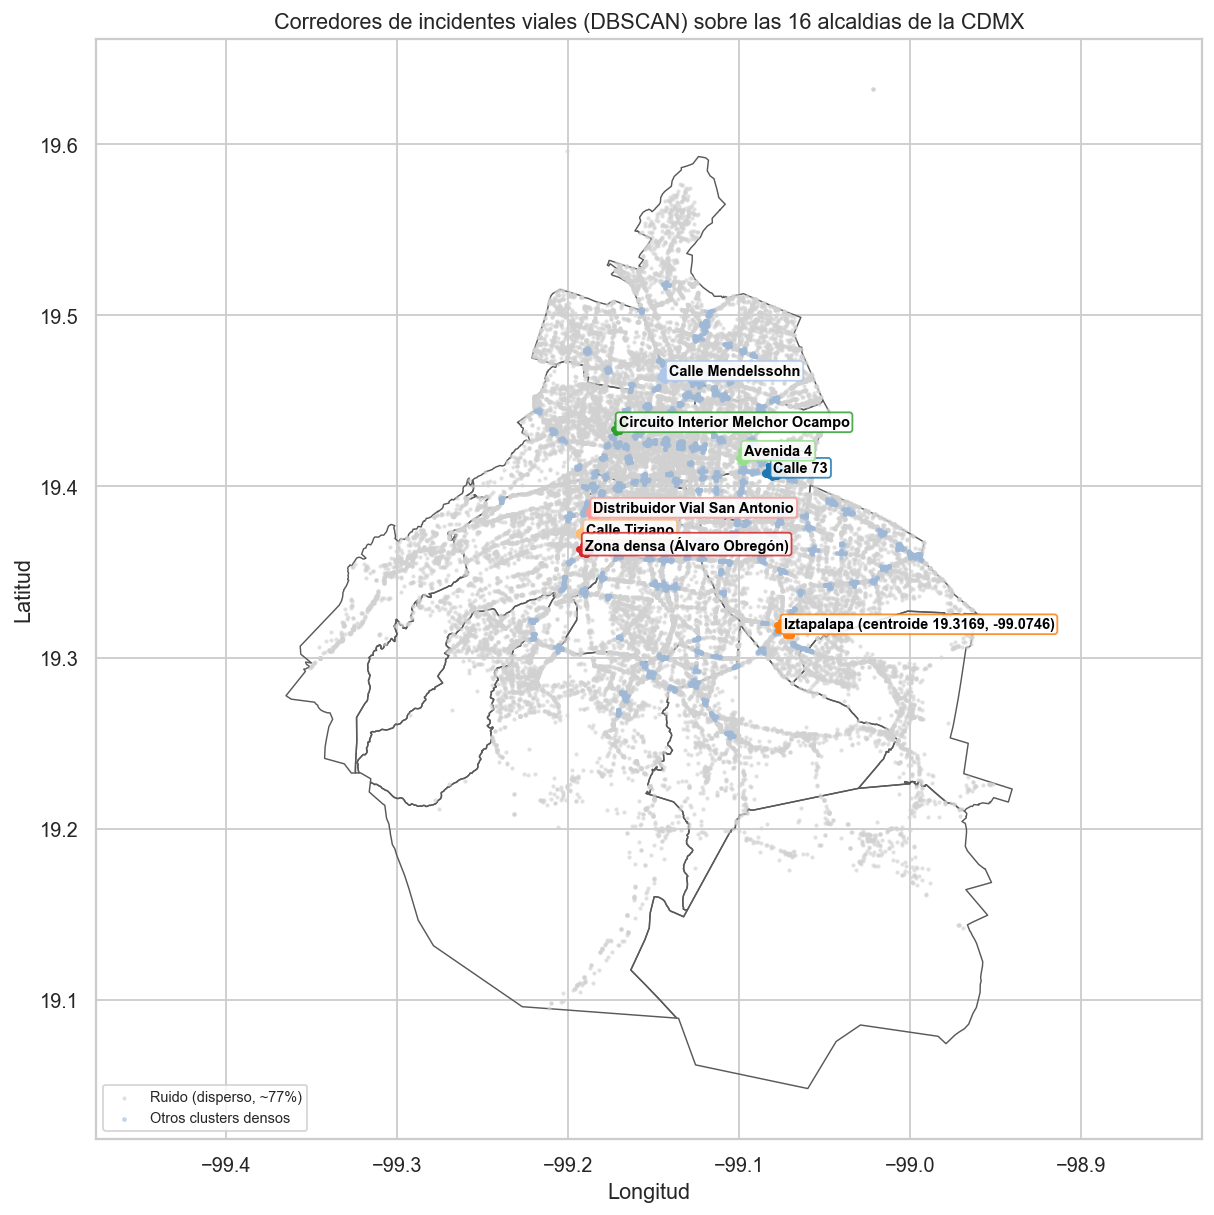
\includegraphics[width=0.9\linewidth]{figura_dbscan_vialidades.png}
\caption{Nodos densos de incidentes sobre la silueta de la CDMX (contorno
oficial de alcaldías). El gris es ruido (incidentes dispersos); los colores son
clusters de DBSCAN, con los principales etiquetados por su vialidad. La versión
\textbf{interactiva} (zoom, paneo y \emph{hover} con vialidad, tipo, alcaldía y
\% real) está en \texttt{figures/mapa\_corredores.html}.}
\label{fig:dbscanmapa}
\end{figure}

\subsection{Evaluación e interpretación}

\textbf{Cohesión interna.} El coeficiente de silueta sobre los puntos no-ruido
(muestra de 20\,000, semilla 42) es \textbf{0.753}: los puntos densos están,
en promedio, mucho más cerca de su propio cluster que del vecino. Los grupos
tienen cohesión y separación reales, no son cortes arbitrarios.

\textbf{Validación externa con el target.} Como \texttt{REAL} nunca participó
en el agrupamiento, comparar el \% afirmativo por cluster contra el global
(63.5\,\%) es una validación externa genuina, con dos hallazgos:
(i) entre los 165 clusters con $n \geq 200$ el \% afirmativo se abre en una
\textbf{banda amplia} —de 40.8\,\% a 89.7\,\% (mediana 59.2\,\%; 52 por encima
del global y 113 por debajo)—, es decir, la \emph{vialidad concreta} sí lleva
señal sobre la veracidad del reporte; y (ii) los nodos densos confirman
\emph{por debajo} del global (58.9\,\% dentro de clusters vs.\ 64.9\,\% en el
ruido): las vialidades de altísimo flujo acumulan proporcionalmente más
reportes falsos/informativos (saturación, llamadas repetidas, sobre-reporte en
hora pico). La implicación operativa es contraintuitiva y valiosa: un reporte
sobre una vialidad saturada merece \emph{más} verificación, no menos.

% ============================================================================
% 8. ARQUITECTURA Y DISEÑO
% ============================================================================
\section{Arquitectura y diseño}

\textbf{Patrón de diseño implementado: Pipeline, en dos niveles.}
(i) \emph{Preparación de datos}: la clase \texttt{PipelinePreparacion}
encadena pasos atómicos de limpieza (\texttt{quitar\_duplicados}
$\rightarrow$ \texttt{quitar\_anio\_ruido} $\rightarrow$
\texttt{construir\_target}), cada uno una función pura
\texttt{df}$\rightarrow$\texttt{df}, y registra una bitácora auditable
(Tabla~\ref{tab:pipe}); agregar, quitar o reordenar un paso es trivial y la
trazabilidad queda impresa. (ii) \emph{Modelado}: el \texttt{Pipeline} de
\texttt{scikit-learn} encadena codificación $\rightarrow$ clasificador en un
único objeto, garantizando que el preprocesamiento ajustado en entrenamiento
se aplique idéntico en validación, prueba y producción —lo que además previene
fugas de preprocesamiento. Se eligió Pipeline porque el procesamiento del
proyecto ocurre naturalmente en etapas secuenciales bien definidas (limpieza
$\rightarrow$ codificación $\rightarrow$ modelo), y el patrón maximiza la
reproducibilidad y la legibilidad del flujo.

\textbf{Diagrama.} La Figura~\ref{fig:arquitectura} muestra el flujo completo:
el pipeline de preparación (nivel i) produce el dataset de trabajo que
consumen los tres notebooks, y el pipeline de modelado (nivel ii) encapsula
preprocesamiento y clasificador en el objeto único que se persiste y recarga.

\begin{figure}[H]\centering
\begin{tikzpicture}[
  font=\small,
  nodo/.style={rectangle, rounded corners=2pt, draw=black!70, fill=blue!8,
               minimum height=8mm, inner sep=5pt, align=center},
  dato/.style={rectangle, draw=black!70, fill=orange!15,
               minimum height=8mm, inner sep=5pt, align=center},
  modelo/.style={rectangle, rounded corners=2pt, draw=black!70, fill=green!12,
               minimum height=8mm, inner sep=5pt, align=center},
  fl/.style={-{Stealth[length=2.5mm]}, thick, black!70},
  etiqueta/.style={font=\footnotesize\itshape, black!60}
]
% ---- Nivel (i): PipelinePreparacion ----
\node[dato] (crudo) {\texttt{c5\_modelado.parquet}\\504\,261 reportes};
\node[nodo, right=9mm of crudo] (p1) {\texttt{quitar\_}\\\texttt{duplicados}};
\node[nodo, right=7mm of p1] (p2) {\texttt{quitar\_}\\\texttt{anio\_ruido}};
\node[nodo, right=7mm of p2] (p3) {\texttt{construir\_}\\\texttt{target}};
\node[dato, right=9mm of p3] (listo) {\texttt{c5\_listo.parquet}\\289\,885 reportes};
\draw[fl] (crudo) -- (p1);
\draw[fl] (p1) -- (p2);
\draw[fl] (p2) -- (p3);
\draw[fl] (p3) -- (listo);
\node[etiqueta, above=2mm of p2] {(i) \texttt{PipelinePreparacion} — bitácora auditable};

% ---- Consumidores ----
\node[nodo, below=11mm of p1, fill=gray!10] (eda) {Notebook 01\\EDA};
\node[modelo, below=11mm of p2.south east] (pipe) {Notebook 02 — \texttt{Pipeline} sklearn\\
  \texttt{ColumnTransformer} $\rightarrow$ \texttt{RandomForest}};
\node[nodo, below=11mm of listo, fill=gray!10] (clu) {Notebook 03\\DBSCAN};
\draw[fl] (listo.south) ++(0,-1mm) |- ($(eda.east)+(0,1mm)$);
\draw[fl] (listo) -- (clu);
\draw[fl] (listo.south) |- ($(pipe.east)+(0,2mm)$);
\node[etiqueta, below=1mm of pipe] {(ii) codificación $\rightarrow$ clasificador en un solo objeto};

% ---- Persistencia ----
\node[dato, below=10mm of pipe.south] (joblib) {\texttt{models/modelo\_rf.joblib} (43 MB)};
\node[modelo, right=8mm of joblib] (demo) {recarga \texttt{joblib.load}\\predicción nueva};
\draw[fl] (pipe.south) ++(0,-5.5mm) -- (joblib);
\draw[fl] (joblib) -- (demo);
\end{tikzpicture}
\caption{Arquitectura del proyecto: el patrón Pipeline en sus dos niveles y la
persistencia/recarga del modelo.}
\label{fig:arquitectura}
\end{figure}

% ============================================================================
% 9. REUTILIZACIÓN DEL MODELO
% ============================================================================
\section{Reutilización del modelo}
\label{sec:reuso}

El modelo final se serializa con \texttt{joblib} en
\texttt{models/modelo\_rf.joblib} (43.1 MB). La última sección del notebook
\texttt{02\_clasificacion.ipynb} lo \textbf{recarga desde disco} —simulando un
servicio que consume el archivo sin reentrenar— y predice reportes nuevos
construidos a mano. La Tabla~\ref{tab:demo} muestra la salida real de la
demostración: el modelo discrimina de forma coherente con el EDA (canales
institucionales y zonas centrales al alza; llamada del 911 en la periferia y
de madrugada a la baja).

\begin{table}[H]
\centering
\caption{Demostración de recarga: predicciones sobre tres reportes nuevos.}
\label{tab:demo}
\small
\begin{tabular}{@{}llllcc@{}}
\toprule
\textbf{Canal} & \textbf{Alcaldía} & \textbf{Incidente} & \textbf{Franja} & \textbf{P(real)} & \textbf{Clase}\\
\midrule
Cámara           & Cuauhtémoc    & Choque con lesionados & Tarde     & 0.806 & REAL\\
Llamada del 911  & Tláhuac       & Choque sin lesionados & Madrugada & 0.355 & falso/inform.\\
Botón de auxilio & Benito Juárez & Choque con lesionados & Mañana    & 0.895 & REAL\\
\bottomrule
\end{tabular}
\end{table}

% ============================================================================
% 10. CONCLUSIONES
% ============================================================================
\section{Conclusiones}

\begin{itemize}[nosep]
  \item \textbf{El \emph{qué} y el \emph{cómo} del reporte predicen su
        veracidad.} El tipo de incidente y el canal de entrada concentran la
        señal del modelo (importancias por permutación 0.102 y 0.031); en el
        análisis bivariado, los canales institucionales confirman $\sim$90\,\%
        frente al $\sim$60\,\% de la llamada del 911, que es el 87.6\,\% del
        volumen.
  \item \textbf{El modelo supera con holgura a la línea base} (F1 macro
        $0.39 \rightarrow 0.66$; AUC 0.73), deteniendo dos de cada tres
        reportes falsos sin colapsar el recall de los reales. El techo de
        desempeño refleja la información limitada disponible al momento del
        reporte, no una falla del algoritmo: la red neuronal comparada empata
        en AUC y pierde en F1 macro.
  \item \textbf{La frontera anti-fuga importa y es demostrable}: incluir el
        tiempo de cierre infla el F1 macro en $+0.06$ de forma espuria; el
        experimento lo cuantifica y justifica el diseño.
  \item \textbf{La confiabilidad tiene geografía y horario}: decae del centro
        a la periferia ($\sim$25 pts entre alcaldías) y de la madrugada a la
        noche (10 pts), siendo las horas de mayor volumen las menos
        confiables.
  \item \textbf{Los incidentes tienen estructura geográfica accionable, pero
        acotada}: DBSCAN encuentra 168 nodos densos (silueta 0.753) que
        concentran solo el 22.7\,\% de los incidentes —cruceros y ejes con
        nombre propio (Circuito Interior, Distribuidor Vial San Antonio,
        Calz.\ Ignacio Zaragoza)— mientras el 77\,\% restante está disperso.
        Y la validación externa revela un matiz contraintuitivo: las
        vialidades más saturadas confirman \emph{por debajo} del promedio
        (58.9\,\% vs.\ 64.9\,\% del ruido), de modo que un reporte en una
        vialidad densa merece más verificación, no menos.
  \item \textbf{Limitaciones}: etiquetado institucional del cierre; ventana
        2022--febrero 2024; sin variables de contexto (clima, tráfico,
        contenido de la llamada). \textbf{Trabajo futuro}: enriquecer las
        llamadas del 911 (donde se concentra el error), calibrar el umbral de
        decisión según el costo operativo del despacho y explorar una zona de
        abstención para derivar los casos ambiguos a verificación humana.
\end{itemize}

% ============================================================================
% 11. REFERENCIAS  (formato APA — mínimo 5)
% ============================================================================
\begin{thebibliography}{9}

\bibitem{c5datos} Gobierno de la Ciudad de México, C5. (2024).
  \emph{Incidentes viales reportados por el C5} [conjunto de datos]. Portal de
  Datos Abiertos de la CDMX. \url{https://datos.cdmx.gob.mx}

\bibitem{melgoza} Melgoza, E., Beltrán-Sánchez, H., \& Vargas Bustamante, A.
  (2023). Injury-related emergency medical service calls, traffic accidents,
  and crime in Mexico City before and during the COVID-19 pandemic.
  \emph{Prehospital and Disaster Medicine, 38}(1), 73--80.
  \url{https://doi.org/10.1017/S1049023X22002230}

\bibitem{herreraortiz} Herrera Ortiz, M. L., Pérez Ferrer, C., Quintero
  Valverde, C., Chías Becerril, L., Martínez Santiago, A., Reséndiz López,
  H. D., Quistberg, D. A., \& Barrientos Gutiérrez, T. (2025). Trends in
  collisions and traffic mortality rates in Mexico City: A comparison of six
  data sources. \emph{PLOS ONE, 20}(10), e0334103.
  \url{https://doi.org/10.1371/journal.pone.0334103}

\bibitem{sklearn} Pedregosa, F., Varoquaux, G., Gramfort, A., et al. (2011).
  Scikit-learn: Machine Learning in Python. \emph{Journal of Machine Learning
  Research, 12}, 2825--2830.
  \url{https://jmlr.org/papers/v12/pedregosa11a.html}

\bibitem{rf} Breiman, L. (2001). Random Forests. \emph{Machine Learning,
  45}(1), 5--32. \url{https://doi.org/10.1023/A:1010933404324}

\bibitem{dbscan} Ester, M., Kriegel, H.-P., Sander, J., \& Xu, X. (1996). A
  Density-Based Algorithm for Discovering Clusters in Large Spatial Databases
  with Noise. \emph{Proceedings of KDD-96}, 226--231.

\bibitem{pandas} McKinney, W. (2010). Data Structures for Statistical
  Computing in Python. \emph{Proceedings of the 9th Python in Science
  Conference}, 56--61. \url{https://doi.org/10.25080/Majora-92bf1922-00a}

\end{thebibliography}

\end{document}
